\chapter{Convolutional Neural Networks}\label{ch:cnn}
\begin{center}\small\textit{Images are not flat vectors -- they have locality, translation, and scale. Convolutions exploit all three.}\end{center}

\noindent\fbox{\parbox{\dimexpr\linewidth-2\fboxsep-2\fboxrule}{%
\textbf{From zero: no vision background assumed.} We start from why MLPs fail on images and build to convolution, pooling, and residual blocks. Every formula is preceded by a picture; kernels and feature maps are defined on first use.}}
\vspace{0.3em}
\section*{Learning Outcomes}
After this chapter you will be able to:
\begin{enumerate}[label=(L\arabic*)]
    \item explain locality, sharing, and translation equivariance of convolutions;
    \item write 2D convolution and count parameters and receptive fields;
    \item describe VGG-to-ResNet blocks and why residuals train deeper;
    \item build a small CNN from scratch and avoid common training pitfalls.
\end{enumerate}

\section{Intuition: Why Not an MLP for Images?}
A $224\times224\times3$ image flattened is $150$k inputs. An MLP hidden layer with 1000 units needs $150$M weights -- huge and blind to structure. Nearby pixels correlate (edges, textures); an object shifted by 10 pixels is still the same object. An MLP must relearn detectors at every position. \textbf{Convolution} shares weights across space: one small filter slides everywhere, detecting the same pattern regardless of location. This gives \textbf{translation equivariance} and drastic parameter savings.

\section{Convolution and Pooling}
\begin{definition}[2D Convolution (cross-correlation)]
Given input $I\in\mathbb{R}^{H\times W}$ and kernel $K\in\mathbb{R}^{k\times k}$,
\begin{equation}
(I*K)_{i,j}=\sum_{u=0}^{k-1}\sum_{v=0}^{k-1} I_{i+u,\,j+v}\,K_{u,v}
\end{equation}
For $C_{\text{in}}$ input channels and $C_{\text{out}}$ filters, $K\in\mathbb{R}^{C_{\text{out}}\times C_{\text{in}}\times k\times k}$. Stride $s$ and padding $p$ control output size: $H_{\text{out}}=\lfloor(H+2p-k)/s\rfloor+1$.
\end{definition}

Pooling downsamples: \textbf{max-pool} takes the max in each $2\times2$ window (stride 2 halves resolution, keeps strongest activation, adds small translation invariance); average-pool smooths.

\begin{center}
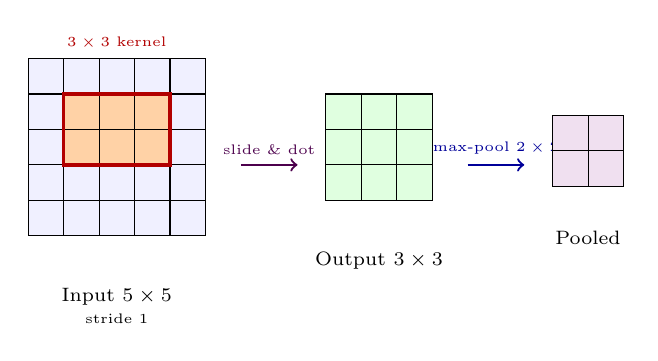
\begin{tikzpicture}[font=\scriptsize, scale=0.90]
  % Input grid 5x5
  \foreach \i in {0,...,4} \foreach \j in {0,...,4} \draw[fill=blue!6] (\i*0.5, -\j*0.5) rectangle ++(0.5,-0.5);
  \foreach \i in {1,2,3} \foreach \j in {1,2} \draw[fill=orange!35] (\i*0.5, -\j*0.5) rectangle ++(0.5,-0.5);
  \draw[very thick, red!70!black] (0.5,-0.5) rectangle ++(1.5,-1.0) node[midway, font=\tiny, text=red!70!black, yshift=1.1cm] {$3\times3$ kernel};
  \node[below, align=center] at (1.25,-3.1) {Input $5\times5$\\{\tiny stride 1}};
  % Arrow
  \draw[->, thick, violet!60!black] (3.0,-1.5) -- (3.8,-1.5) node[midway, above, font=\tiny] {slide \& dot};
  % Output 3x3
  \foreach \i in {0,...,2} \foreach \j in {0,...,2} \draw[fill=green!12] (4.2+\i*0.5, -\j*0.5-0.5) rectangle ++(0.5,-0.5);
  \node[below, align=center] at (4.95,-2.6) {Output $3\times3$};
  % Pool
  \draw[->, thick, blue!60!black] (6.2,-1.5) -- (7.0,-1.5) node[midway, above, font=\tiny] {max-pool $2\times2$};
  \foreach \i in {0,1} \foreach \j in {0,1} \draw[fill=violet!12] (7.4+\i*0.5, -\j*0.5-0.8) rectangle ++(0.5,-0.5);
  \node[below, align=center] at (7.9,-2.3) {Pooled};
\end{tikzpicture}
\end{center}

A CNN stacks: \texttt{Conv $\to$ BatchNorm $\to$ ReLU $\to$ Pool}, repeating. Early layers learn Gabor-like edge detectors; deeper layers compose them into textures, parts, objects -- a learned hierarchy.

\section{Classic Architectures to ResNet}
\begin{itemize}
\item \textbf{LeNet-5} (1998): 2 conv+pool + 3 FC -- reads digits.
\item \textbf{AlexNet} (2012): 5 conv + 3 FC, ReLU, dropout, GPU -- wins ImageNet, sparks deep learning boom.
\item \textbf{VGG} (2014): only $3\times3$ conv, deeper (16--19 layers) -- simplicity.
\item \textbf{GoogLeNet/Inception}: parallel multi-scale filters.
\item \textbf{ResNet} (2015): solves degradation (deeper nets got \emph{worse}) via skip connections.
\end{itemize}

\begin{definition}[Residual Block]
Instead of learning $\mathcal{H}(\mathbf{x})$, learn residual $\mathcal{F}(\mathbf{x})=\mathcal{H}(\mathbf{x})-\mathbf{x}$:
\begin{equation}
\mathbf{y}=\mathcal{F}(\mathbf{x},\{W_i\})+\mathbf{x}
\end{equation}
If identity is optimal, the net can push $\mathcal{F}\to0$ (easy) rather than fit identity through non-linear layers (hard). Gradient flows directly through the skip, curing vanishing gradients.
\end{definition}

\begin{center}
\begin{tikzpicture}[font=\scriptsize, >=Stealth, scale=0.93]
  \node[draw, fill=blue!12, rounded corners, minimum width=1.4cm, minimum height=0.7cm] (in) at (0,0) {$\mathbf{x}$};
  \node[draw, fill=green!12, rounded corners, minimum width=1.6cm, minimum height=0.7cm] (c1) at (3,0.6) {Conv $3\times3$};
  \node[draw, fill=green!12, rounded corners, minimum width=1.6cm, minimum height=0.7cm] (c2) at (3,-0.8) {Conv $3\times3$};
  % Actually need two in series with skip
  \node[draw, fill=orange!12, circle, minimum size=0.7cm] (add) at (6,0) {$+$};
  \node[draw, fill=violet!12, rounded corners, minimum width=1.0cm, minimum height=0.7cm] (relu) at (7.8,0) {ReLU};
  \draw[->, thick, blue!60!black] (in) -- (c1);
  \draw[->, thick] (c1) -- (c2);
  \draw[->, thick] (c2) -- (add);
  \draw[->, thick, red!70!black, bend left=22] (in) to node[above, font=\tiny] {skip / identity} (add);
  \draw[->, thick] (add) -- (relu);
  \node[below, font=\tiny, text=gray!60!black, align=center] at (3,-1.6) {$\mathcal{F}(\mathbf{x})$\\{\tiny 2 conv + BN + ReLU}};
  \node[above, font=\tiny, text=violet!70!black] at (7.8,0.6) {$\mathbf{y}$};
\end{tikzpicture}
\end{center}

ResNet-18/50/152 stack such blocks, reaching 100+ layers with \emph{lower} training error than 20-layer nets -- depth finally helps. BatchNorm inside each block stabilizes.

\section{Worked Example: CNN from Scratch}
\begin{example}[PyTorch CNN for CIFAR-10]
\begin{lstlisting}[language=Python]
import torch.nn as nn
class TinyCNN(nn.Module):
    def __init__(self):
        super().__init__()
        self.features = nn.Sequential(
            nn.Conv2d(3,32,3,padding=1), nn.BatchNorm2d(32), nn.ReLU(),
            nn.MaxPool2d(2),  # 32 -> 16
            nn.Conv2d(32,64,3,padding=1), nn.BatchNorm2d(64), nn.ReLU(),
            nn.MaxPool2d(2),  # 16 -> 8
            nn.Conv2d(64,128,3,padding=1), nn.BatchNorm2d(128), nn.ReLU(),
            nn.AdaptiveAvgPool2d(1)  # -> (128,1,1)
        )
        self.classifier = nn.Linear(128, 10)
    def forward(self, x):
        x = self.features(x).flatten(1)
        return self.classifier(x)

# Residual block
class ResBlock(nn.Module):
    def __init__(self, c):
        super().__init__()
        self.conv1 = nn.Conv2d(c,c,3,padding=1,bias=False)
        self.bn1 = nn.BatchNorm2d(c)
        self.conv2 = nn.Conv2d(c,c,3,padding=1,bias=False)
        self.bn2 = nn.BatchNorm2d(c)
    def forward(self, x):
        out = torch.relu(self.bn1(self.conv1(x)))
        out = self.bn2(self.conv2(out))
        return torch.relu(out + x)  # skip connection

# Count params: TinyCNN ~ 100k, ResNet-18 ~ 11M
model = TinyCNN()
print(f"Params: {sum(p.numel() for p in model.parameters())}")
\end{lstlisting}
\end{example}

A pure NumPy convolution inner loop is also instructive:
\begin{center}
\begin{lstlisting}[language=Python]
import numpy as np
def conv2d_numpy(img, kernel):
    H,W = img.shape; kH,kW = kernel.shape
    out = np.zeros((H-kH+1, W-kW+1))
    for i in range(out.shape[0]):
        for j in range(out.shape[1]):
            out[i,j] = np.sum(img[i:i+kH, j:j+kW] * kernel)
    return out

# Sobel edge detector
sobel_x = np.array([[-1,0,1],[-2,0,2],[-1,0,1]], dtype=float)
edges = conv2d_numpy(np.random.randn(28,28), sobel_x)
\end{lstlisting}
\end{center}

\section{Vision Beyond Classification}
CNN features transfer: the same backbone serves detection (Faster R-CNN, YOLO -- bounding boxes), segmentation (U-Net -- per-pixel masks), and self-supervised pretraining. Modern vision mixes CNNs with Transformers (ViT), but convolution remains the efficient inductive bias for grid data.

\section{Receptive Field and Parameter Counting}
A $3\times3$ conv has $9C_{in}C_{out}$ weights -- independent of image size.
Stacking two $3\times3$ layers yields a $5\times5$ receptive field with fewer
parameters ($2\cdot9$ vs $25$ per channel) and an extra non-linearity. After
$L$ layers of stride 1, receptive field $=1+L(k-1)$. Stride or pooling
exponentially expands it. Dilated (atrous) conv inserts gaps to grow field
without downsampling -- vital for segmentation.

\section{Translation Equivariance Proof Sketch}
Let $T_{\Delta}$ shift input by $\Delta$. Then $(T_{\Delta}I)*K = T_{\Delta}(I*K)$
because summation indices shift uniformly -- convolution commutes with
translation. Pooling is approximately invariant: $\text{Pool}(T_{\Delta}I)\approx
\text{Pool}(I)$ for $|\Delta|<$ pool window, giving robustness to small jitters.
Fully-connected layers lack this property, hence CNNs need far less data for
vision.

\section{Architectures in Detail: VGG to ResNet to EfficientNet}
VGG showed depth matters; GoogLeNet showed multi-scale matters. ResNet made
depth \emph{trainable}: 152 layers beat 34, and 1001-layer ResNets were trained.
Follow-ups: \textbf{DenseNet} concatenates all prior feature maps; \textbf{ResNeXt}
adds grouped conv; \textbf{EfficientNet} compound-scales width/depth/resolution
with neural architecture search. All retain convolution as the workhorse; recent
hybrids replace late conv stages with Transformer blocks (CoAtNet).

\section{Efficient CNN Training Tricks}
Use He init, BatchNorm after conv (before ReLU), weight decay $10^{-4}$, SGD
with momentum $0.9$ and cosine decay, label smoothing $0.1$, and Mixup/CutMix.
Progressive resizing (start $128^2$, end $224^2$) speeds training. Depthwise
separable conv (MobileNet) factorizes $k\times k\times C_{in}\times C_{out}$
into $k\times k\times C_{in}$ (spatial) + $1\times1\times C_{in}\times C_{out}$
(pointwise) for $8$--$9\times$ savings on mobile.

\section{Common Pitfalls}
Forgetting padding causes spatial shrinkage and border artifacts -- use
\texttt{padding=1} for $3\times3$ stride 1 to preserve size. Not normalizing
inputs (ImageNet mean/std) slows convergence by an order of magnitude. Using
large $7\times7$ kernels where two $3\times3$ suffice wastes compute. And
placing dropout before BatchNorm is unstable -- order matters: Conv $\to$ BN
$\to$ ReLU $\to$ Dropout (or use DropBlock for conv).

\section{Further Reading}
LeCun et al. (1998) LeNet; Krizhevsky et al. (2012) AlexNet; Simonyan \&
Zisserman (2014) VGG; He et al. (2016) ResNet. For modern practice, see
Howard \& Gugger, \emph{Deep Learning for Coders}, and the \texttt{timm}
library -- every architecture in one repo, ideal for ablations.

\section{Chapter Summary}
Convolutions share weights spatially: $k\times k$ filters slide, giving
translation equivariance and $O(k^2C_{in}C_{out})$ params. Pooling downsamples
and adds invariance. Stacking yields hierarchical features; residuals let depth
scale to 100+ layers. ResNet's $\mathbf{y}=\mathcal{F}(\mathbf{x})+\mathbf{x}$
is the trick that unlocked depth. The same conv backbone powers detection,
segmentation, and beyond.

\smallskip
\noindent\textit{Key takeaways:} (1) conv $=$ local + shared + equivariant;
(2) pooling $\approx$ invariant; (3) receptive field grows linearly then
exponentially; (4) ResNet skip cures degradation; (5) depthwise separable
conv saves $8\times$ for mobile.

\section{Exercises}
\begin{exercise} Compute output size for input $32\times32\times3$, kernel $5\times5$, stride 1, padding 2, 16 filters. How many parameters (with bias)? Compare to an MLP with same output dimension.\end{exercise}
\begin{exercise} Prove convolution is translation equivariant: shifting input then convolving equals convolving then shifting. Why is pooling \emph{invariant} (approximately)?\end{exercise}
\begin{exercise} Implement NumPy max-pool $2\times2$ stride 2. Test on a $4\times4$ matrix and verify gradients route only to max positions.\end{exercise}
\begin{exercise} Build a ResBlock and show that if weights are zero, it computes identity. Explain why this makes optimization easier than a plain stack.\end{exercise}
\begin{exercise} Train TinyCNN on CIFAR-10 for 5 epochs. Replace AdaptiveAvgPool with Flatten+Linear and compare parameter counts and accuracy. When does global average pooling help?\end{exercise}
% End of Chapter
